\section{Introduction}

\begin{frame}{From frozen prior to learned basis}
	\vspace{-5pt}
	\textbf{1st hybridization:} neural prior trained offline, then \coloredonly<1>{frozen}: a priori error estimates.

	\textbf{Limit:} the gain is bounded by the \coloredonly<1>{quality of the prior}, trained apart from the scheme.

	% pas d'environnement center : ses espaces (\topsep) sont compressibles et la 1re figure remontait à l'overlay 2, quand la slide devient pleine
	\vspace{-5pt}
	{\centering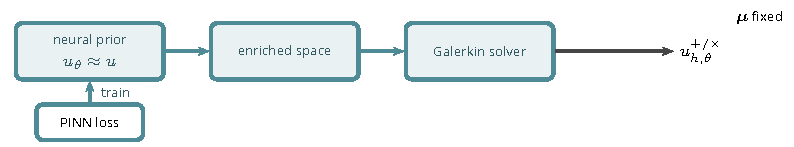
\includegraphics[page=1]{images/contrib2/transition/transition.pdf}\par}

	\vspace{2pt}
	\blk*{2}{%
		\textbf{2nd hybridization:} learn the basis \coloredonly<2>{through the solver}, adapted to the solution of the scheme.

		\textbf{Advantage:} basis adapted to the scheme, \coloredonly<2>{not bounded by a frozen prior}.

		\textbf{Limit:} \coloredonly<2>{no a priori guarantees}, training cost.
	}

	\only<2>{%
		\vspace{-5pt}
		{\centering\includegraphics[page=2]{images/contrib2/transition/transition.pdf}\par}
	}%

\end{frame}